\paragraph*{Historical and layer-wise attention structure.}
Figures~\ref{fig:attn-temporal}--\ref{fig:attn-horizons} examine temporal context within the same supplementary mixed-disturbance analysis. Figure~\ref{fig:attn-temporal} covers all 30 historical windows under normal and upcoming conditions, with an upcoming-minus-normal panel that resolves smaller shifts in the historical positions receiving attention. Its difference scale is much narrower than the absolute-weight scale, so the panel should not be read as a large change in temporal dependence. Figure~\ref{fig:attn-layers} focuses the main-text comparison on encoder layers 1, 4, and 5, retaining an input-near layer and the final two layers while keeping both geographic and semantic branches readable. The complete five-layer view is retained in Appendix~\ref{app:layerwise-attention}. Layer-specific weights do not measure the accuracy contribution of each layer.

Figure~\ref{fig:attn-horizons} compares the upcoming-minus-normal resource maps from three separately trained Start$\leq5/10/15$ mixed-disturbance checkpoints, with 96 samples per condition and checkpoint. The persistent structure and localized changes provide a descriptive view across onset settings. They neither trace propagation through physical time nor replace the distance-resolved recall comparison in Table~\ref{tab:delay-ablation-new}.
\zhpara{图~\ref{fig:attn-temporal}--图~\ref{fig:attn-horizons}从历史时间、编码层和起点范围三个角度展开混合扰动补充分析。时间图覆盖三十个历史窗口，比较正常与即将形成瓶颈两种状态，并以差值图呈现较小的历史位置重分配；其差值色标远窄于绝对权重色标，因此不能把颜色对比理解为时间依赖发生剧烈变化。正文逐层图聚焦编码器第 1、4、5 层，保留靠近输入的一层及最后两层，并同时展示地理与语义分支；完整五层结果保留在附录~\ref{app:layerwise-attention}。层级权重本身不量化各层对准确率的贡献。跨范围图比较分别训练的五分钟、十分钟和十五分钟 checkpoint，每种状态、每个 checkpoint 选取九十六个样本。图中的结构与局部变化用于描述不同预测设置下的信息分配，并不等同于物理时间上的传播过程；延迟建模收益仍由表~\ref{tab:delay-ablation-new}中的距离分解召回支持。}
\begin{figure*}[t]
\centering
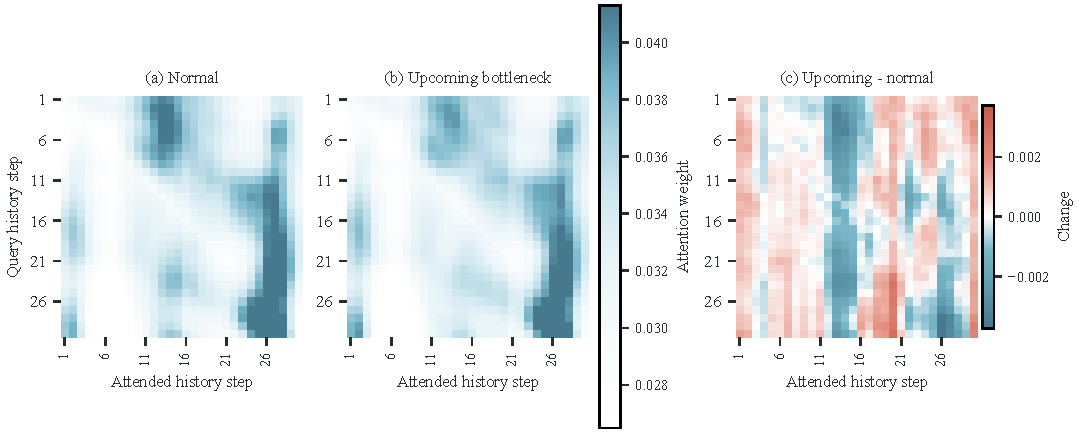
\includegraphics[width=0.98\textwidth]{figures/attention_heatmaps/fig04_temporal_attention_states.pdf}
\caption{Temporal attention over the 30 historical windows under normal and upcoming conditions, with upcoming-minus-normal change. Weights are averaged across selected samples, resources, heads and layers. Absolute and difference panels use separate scales. Mixed-disturbance supplementary analysis (\texttt{dense\_i1\_mix}, seed 42); not the retained \texttt{dense\_i1} evaluation.}
\label{fig:attn-temporal}
\end{figure*}
\begin{figure*}[t]
\centering
\includegraphics[width=0.92\textwidth]{figures/attention_heatmaps/fig05_layerwise_upcoming_attention_selected.pdf}
\caption{Geographic (upper row) and semantic (lower row) attention in selected encoder layers 1, 4, and 5 for upcoming samples. Each row uses the same scale as the complete five-layer view in Appendix~\ref{app:layerwise-attention}; the two branches have separate scales. Start cap 5 min, 96 samples. Mixed-disturbance supplementary analysis (\texttt{dense\_i1\_mix}, seed 42); not the retained \texttt{dense\_i1} evaluation.}
\label{fig:attn-layers}
\end{figure*}
\begin{figure*}[p]
\centering
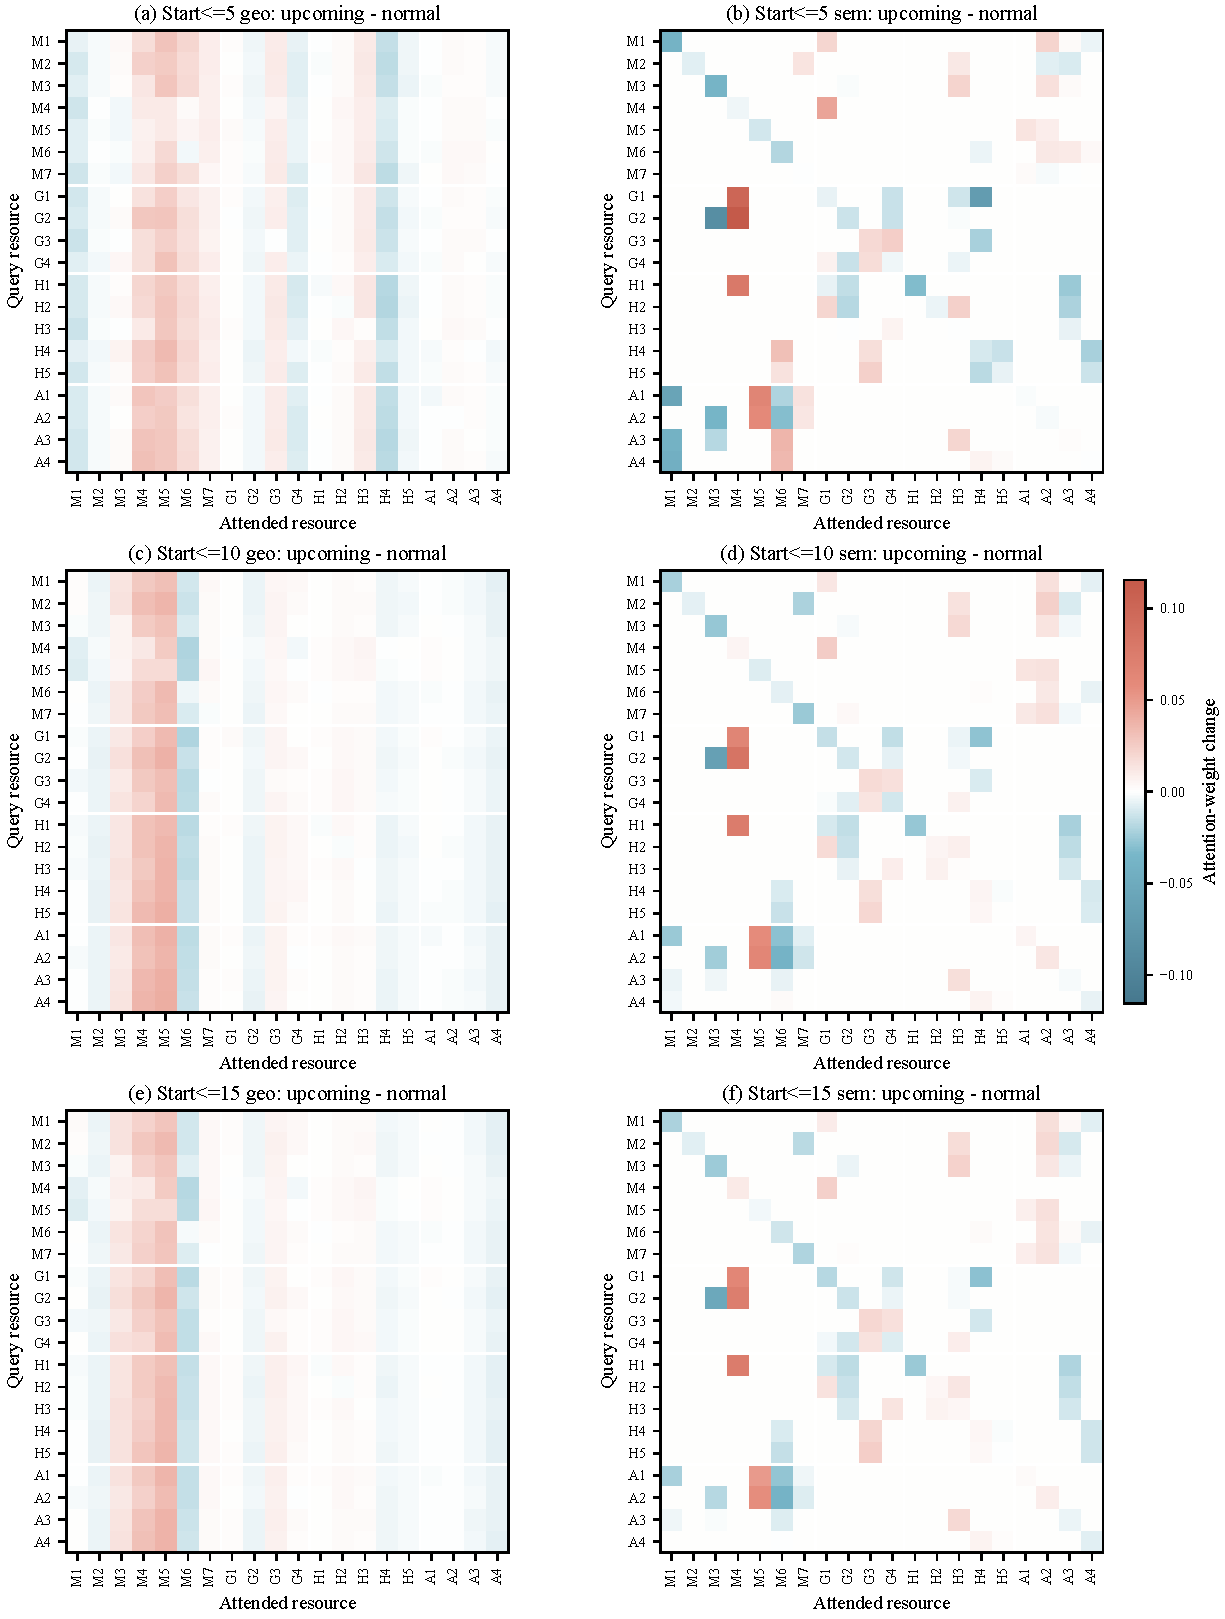
\includegraphics[width=0.98\textwidth]{figures/attention_heatmaps/fig07_horizon_attention_change.pdf}
\caption{Upcoming-minus-normal attention change across separately trained Start cap 5, 10 and 15 min checkpoints. Upper row (a,c,e): geographic; lower row (b,d,f): semantic. All panels share one signed scale; they are not repeated-seed estimates or a physical propagation sequence. Mixed-disturbance supplementary analysis (\texttt{dense\_i1\_mix}, seed 42); not the retained \texttt{dense\_i1} evaluation.}
\label{fig:attn-horizons}
\end{figure*}
